\section{Stronger Attackers, Classical Traffic Controls and Power Planning (E14)}\label{sec:r7-supp}
E14 is a post hoc sensitivity analysis of the existing cohort. It reuses E13's six measured conditions and adds seven offline transformations of its undefended captures, all on the same 414 training and 276 test trajectories. No new customer, model decision or packet measurement is produced by these transformations. The configuration and source hashes were frozen before fitting the new attacks; the source cohort and its earlier outcomes were already known. All configurations are reported.

\subsection{Defense-aware attacker expansion}
The primary attacker is $D_2$: it knows the algorithm and parameter distribution and fits on training examples generated under the evaluated defense. Seven R7 models comprise a majority control, logistic regression, gradient boosting, random forest, extra trees, a k-FP-style forest-leaf nearest-neighbor attack \cite{hayes2016kfp}, and a trainable 1D-CNN. This leaf adaptation uses 200 trees and Hamming-distance three-nearest-neighbor voting on training leaf fingerprints, not an exact reproduction of the original k-FP extractor. Tabular inputs contain full-trace counts, sizes, time summaries, directional bursts and sampled cumulative signed sizes. None includes tool names, labels, customer IDs, real/cover markers or test outcomes. The CNN uses direction, log length, log interarrival and a mask; its two convolutional layers have 16/32 channels, followed by mean/max pooling and a binary head. It is trained for 50 fixed epochs with Adam, learning rate .001 and class-weighted loss. The first/last halves of sequences longer than 512 records are retained; Table~\ref{tab:r7-all} reports truncation. Other learners preserve full-trace aggregate counts. Models and hashes are saved before test scoring. No test-guided hyperparameter selection is performed in this extension.

For measured conditions, the entire original E13 union remains included: size/order, timing, joint, training-derived profile decoding and learned flush stripping. The maximum therefore cannot decrease merely because a weaker new learner replaces an old one. Each of 2,000 common customer-bootstrap draws reselects the maximum. Draws missing a target class are excluded (counts are saved per cell). The intervals condition on fitted predictions and are not bounds against arbitrary future attackers. No expanded cell meets the original absolute criterion; the threshold is unchanged.

\subsection{Classical WF mechanisms adapted to RPC traces}
Every offline adapter tracks abstract fragments derived from input record sizes and verifies no loss, reordering or scheduling before release. This checks metadata and byte accounting, not payload-content equality or actual delivery. Fixed cells use 512 plaintext bytes plus 24 TLS~1.2 AEAD bytes and the five-byte header. Fragment IDs are excluded from attack inputs. All controls use the same held-out trajectories and byte accounting; they are not Tor deployments and do not inherit a published implementation's accuracy or guarantees.

Tamaraw uses constant per-direction slots, 40/12\,ms or 4/1.2\,ms, and randomized geometric padding to multiples of 50 cells \cite{cai2014systematic}. Input-order queueing propagates waits to subsequent real fragments. FRONT draws a uniform dummy budget and a Rayleigh schedule per direction and cancels outstanding dummies when the real trace ends \cite{gong2020front}; the budget is the training median cell count and the window spans training-duration quartiles. The shifted calibration fits those values only on the shorter half of training customers; D2 attackers still use all defended training customers and every test customer remains included. This is an in-population calibration stress test, not evidence of cross-environment transfer.

The WTF-PAD mechanism adaptation retains send/receive triggers, burst/gap/wait states, token removal/refill and infinity outcomes \cite{juarez2016wtfpad}. It uses an empirical training interarrival histogram, burst/gap infinity probabilities .1/.25, real-event reset and a 64-dummy-per-gap cap, rather than reproducing the public simulator's fitted log-normal Tor configuration. Walkie-Talkie molds half-duplex burst lengths with a random training donor from another customer and adds donor-only tail bursts \cite{wang2017walkietalkie}. It has no sensitive/non-sensitive symmetric pairing oracle and therefore does not inherit that pairing's indistinguishability argument. These exact adaptations and their limits are documented with the executable source.

\subsection{Results and cost interpretation}
The strongest learner depends on the operating point: the new CNN increases some tunnel BAs and supports inference on several classical controls; the forest-leaf attack improves the record-bucket return attack. The serial-shadow timing signal remains, so the earlier clock-boundary finding survives this expansion. The alternative WF points can reduce byte/tool-call cost substantially, precluding a claim that shadow cover is universally superior. The shorter-calibration FRONT result does not degrade monotonically: all points and both prompt arms are retained rather than selecting the direction expected by the hypothesis.

\begin{longtable}{@{}llrrrr@{}}
\caption{E14: all prompt/defense cells, maximum over the expanded attack suite. Customer bootstrap 95\% BA intervals; AUC is suite-maximum AUROC. All 52 cells fail the absolute criterion.}\label{tab:r7-all}\\
\toprule Prompt / condition & Target & BA [95\% CI] & AUC & Attacks & CNN trunc.\\\midrule\endfirsthead
\toprule Prompt / condition & Target & BA [95\% CI] & AUC & Attacks & CNN trunc.\\\midrule\endhead
Standard / Undefended & cancel & 91.7 [84.7, 100.0] & 0.917 & 19 & 0\\
Standard / Undefended & return & 86.4 [79.5, 97.2] & 0.875 & 19 & 0\\
Standard / Per-call constant & cancel & 68.6 [51.4, 92.8] & 0.678 & 19 & 0\\
Standard / Per-call constant & return & 62.7 [54.2, 79.5] & 0.657 & 19 & 0\\
Standard / Serial shadow & cancel & 61.4 [54.6, 71.4] & 0.625 & 22 & 0\\
Standard / Serial shadow & return & 53.4 [50.3, 65.8] & 0.530 & 22 & 0\\
Standard / Two-in-flight shadow & cancel & 51.7 [50.0, 69.1] & 0.554 & 22 & 0\\
Standard / Two-in-flight shadow & return & 57.7 [56.6, 69.7] & 0.596 & 22 & 0\\
Standard / Full tunnel, 2 ms & cancel & 62.5 [57.6, 70.2] & 0.708 & 17 & 0\\
Standard / Full tunnel, 2 ms & return & 55.2 [51.9, 62.0] & 0.569 & 17 & 0\\
Standard / Full tunnel, 5 ms & cancel & 54.6 [51.4, 72.9] & 0.618 & 17 & 0\\
Standard / Full tunnel, 5 ms & return & 57.3 [54.2, 64.2] & 0.555 & 17 & 0\\
Standard / Record buckets & cancel & 53.1 [50.0, 78.5] & 0.510 & 7 & 0\\
Standard / Record buckets & return & 69.8 [50.0, 86.9] & 0.689 & 7 & 0\\
Standard / Tamaraw 40/12 ms & cancel & 55.3 [50.0, 68.7] & 0.590 & 7 & 2\\
Standard / Tamaraw 40/12 ms & return & 55.3 [51.1, 64.4] & 0.594 & 7 & 2\\
Standard / Tamaraw 4/1.2 ms & cancel & 57.8 [50.0, 71.8] & 0.609 & 7 & 1\\
Standard / Tamaraw 4/1.2 ms & return & 51.8 [50.0, 61.8] & 0.525 & 7 & 1\\
Standard / FRONT & cancel & 59.0 [50.0, 69.9] & 0.623 & 7 & 0\\
Standard / FRONT & return & 69.3 [58.3, 81.8] & 0.713 & 7 & 0\\
Standard / WTF-PAD adaptation & cancel & 51.9 [50.0, 64.1] & 0.560 & 7 & 0\\
Standard / WTF-PAD adaptation & return & 62.7 [50.0, 79.6] & 0.635 & 7 & 0\\
Standard / WT random-donor & cancel & 50.0 [50.0, 67.0] & 0.526 & 7 & 0\\
Standard / WT random-donor & return & 56.7 [51.7, 67.8] & 0.607 & 7 & 0\\
Standard / FRONT, short calibration & cancel & 52.4 [50.0, 61.3] & 0.546 & 7 & 0\\
Standard / FRONT, short calibration & return & 56.0 [50.0, 71.1] & 0.618 & 7 & 0\\
Rules / Undefended & cancel & 94.4 [83.3, 100.0] & 0.944 & 19 & 0\\
Rules / Undefended & return & 87.0 [78.4, 97.6] & 0.905 & 19 & 0\\
Rules / Per-call constant & cancel & 70.1 [50.0, 86.0] & 0.680 & 19 & 0\\
Rules / Per-call constant & return & 61.9 [50.8, 78.0] & 0.563 & 19 & 0\\
Rules / Serial shadow & cancel & 58.2 [53.8, 76.3] & 0.589 & 22 & 0\\
Rules / Serial shadow & return & 60.7 [57.1, 72.6] & 0.626 & 22 & 0\\
Rules / Two-in-flight shadow & cancel & 56.9 [51.9, 70.4] & 0.580 & 22 & 0\\
Rules / Two-in-flight shadow & return & 60.2 [55.4, 73.9] & 0.639 & 22 & 0\\
Rules / Full tunnel, 2 ms & cancel & 53.1 [51.7, 65.7] & 0.504 & 17 & 0\\
Rules / Full tunnel, 2 ms & return & 59.1 [55.3, 67.6] & 0.590 & 17 & 0\\
Rules / Full tunnel, 5 ms & cancel & 58.3 [50.0, 67.9] & 0.539 & 17 & 0\\
Rules / Full tunnel, 5 ms & return & 56.3 [55.7, 64.0] & 0.595 & 17 & 0\\
Rules / Record buckets & cancel & 56.7 [50.0, 81.2] & 0.615 & 7 & 0\\
Rules / Record buckets & return & 70.8 [51.2, 88.0] & 0.703 & 7 & 0\\
Rules / Tamaraw 40/12 ms & cancel & 58.6 [56.3, 70.8] & 0.622 & 7 & 0\\
Rules / Tamaraw 40/12 ms & return & 50.0 [50.0, 60.3] & 0.500 & 7 & 0\\
Rules / Tamaraw 4/1.2 ms & cancel & 52.5 [50.0, 61.6] & 0.505 & 7 & 3\\
Rules / Tamaraw 4/1.2 ms & return & 54.6 [51.4, 61.5] & 0.534 & 7 & 3\\
Rules / FRONT & cancel & 58.5 [50.0, 69.6] & 0.544 & 7 & 0\\
Rules / FRONT & return & 60.4 [50.0, 75.1] & 0.635 & 7 & 0\\
Rules / WTF-PAD adaptation & cancel & 57.2 [50.0, 74.2] & 0.559 & 7 & 0\\
Rules / WTF-PAD adaptation & return & 61.0 [50.0, 77.6] & 0.625 & 7 & 0\\
Rules / WT random-donor & cancel & 51.4 [50.0, 68.8] & 0.606 & 7 & 0\\
Rules / WT random-donor & return & 56.3 [50.0, 66.6] & 0.558 & 7 & 0\\
Rules / FRONT, short calibration & cancel & 51.2 [50.0, 70.1] & 0.501 & 7 & 0\\
Rules / FRONT, short calibration & return & 62.9 [50.0, 77.2] & 0.655 & 7 & 0\\
\bottomrule\end{longtable}


\subsection{Matched-suite cost sensitivity}
The strongest-available union contains 17--22 attacks for measured conditions and seven for offline controls. Maxima over these unequal unions cannot by themselves establish a matched-attacker dominance relation. We therefore recompute all cells using exactly the seven common R7 models, without new fitting (Table~\ref{tab:r7-common}). Figure~\ref{fig:r7-pareto} uses this matched subset; its gray upper endpoints retain the larger available unions. For example, standard-prompt serial shadow changes from 61.4/53.4\% under its full union to 50.0/52.9\% under the common subset, while WT remains 50.0/56.7\%. WT's lower byte cost then trades off against higher worst-target BA, rather than dominating serial shadow. The serial timing finding from the full suite remains unchanged. One subset cell (standard-prompt, two-in-flight shadow, cancellation) meets the gate, but its full-union cell does not; restricting the comparison suite does not certify the defense. This sensitivity separates matched cost comparisons from the strongest observed attack evidence.
\begin{longtable}{@{}llrrrr@{}}
\caption{Matched-suite sensitivity: the same seven R7 models in every E14 condition. BA and AUROC maxima are independently reselected in every customer-bootstrap draw. This subset is used for the cost plot, not to replace the stronger available attack union or its absolute assessment.}\label{tab:r7-common}\\
\toprule Prompt / condition & Target & BA [95\% CI] & AUROC & Valid draws & Subset gate\\\midrule\endfirsthead
\toprule Prompt / condition & Target & BA [95\% CI] & AUROC & Valid draws & Subset gate\\\midrule\endhead
Standard / Undefended & cancel & 84.3 [72.7, 97.4] & 0.836 & 1988 & Unmet\\
Standard / Undefended & return & 76.9 [62.2, 90.4] & 0.828 & 2000 & Unmet\\
Standard / Per-call constant & cancel & 53.2 [50.0, 69.5] & 0.604 & 1988 & Unmet\\
Standard / Per-call constant & return & 59.1 [50.0, 73.8] & 0.656 & 2000 & Unmet\\
Standard / Serial shadow & cancel & 50.0 [50.0, 65.0] & 0.548 & 1988 & Unmet\\
Standard / Serial shadow & return & 52.9 [50.0, 60.3] & 0.526 & 2000 & Unmet\\
Standard / Two-in-flight shadow & cancel & 50.0 [50.0, 59.7] & 0.500 & 1988 & Pass\\
Standard / Two-in-flight shadow & return & 57.3 [55.0, 69.2] & 0.596 & 2000 & Unmet\\
Standard / Full tunnel, 2 ms & cancel & 59.9 [54.6, 67.3] & 0.708 & 1988 & Unmet\\
Standard / Full tunnel, 2 ms & return & 55.2 [50.1, 61.0] & 0.567 & 2000 & Unmet\\
Standard / Full tunnel, 5 ms & cancel & 54.6 [50.0, 70.5] & 0.618 & 1988 & Unmet\\
Standard / Full tunnel, 5 ms & return & 53.7 [51.3, 61.2] & 0.551 & 2000 & Unmet\\
Standard / Record buckets & cancel & 53.1 [50.0, 78.5] & 0.510 & 1988 & Unmet\\
Standard / Record buckets & return & 69.8 [50.0, 86.9] & 0.689 & 2000 & Unmet\\
Standard / Tamaraw 40/12 ms & cancel & 55.3 [50.0, 68.7] & 0.590 & 1988 & Unmet\\
Standard / Tamaraw 40/12 ms & return & 55.3 [51.1, 64.4] & 0.594 & 2000 & Unmet\\
Standard / Tamaraw 4/1.2 ms & cancel & 57.8 [50.0, 71.8] & 0.609 & 1988 & Unmet\\
Standard / Tamaraw 4/1.2 ms & return & 51.8 [50.0, 61.8] & 0.525 & 2000 & Unmet\\
Standard / FRONT & cancel & 59.0 [50.0, 69.9] & 0.623 & 1988 & Unmet\\
Standard / FRONT & return & 69.3 [58.3, 81.8] & 0.713 & 2000 & Unmet\\
Standard / WTF-PAD adaptation & cancel & 51.9 [50.0, 64.1] & 0.560 & 1988 & Unmet\\
Standard / WTF-PAD adaptation & return & 62.7 [50.0, 79.6] & 0.635 & 2000 & Unmet\\
Standard / WT random-donor & cancel & 50.0 [50.0, 67.0] & 0.526 & 1988 & Unmet\\
Standard / WT random-donor & return & 56.7 [51.7, 67.8] & 0.607 & 2000 & Unmet\\
Standard / FRONT, short calibration & cancel & 52.4 [50.0, 61.3] & 0.546 & 1988 & Unmet\\
Standard / FRONT, short calibration & return & 56.0 [50.0, 71.1] & 0.618 & 2000 & Unmet\\
Rules / Undefended & cancel & 84.7 [75.2, 98.5] & 0.851 & 1988 & Unmet\\
Rules / Undefended & return & 78.3 [63.3, 92.2] & 0.818 & 2000 & Unmet\\
Rules / Per-call constant & cancel & 59.4 [50.0, 77.5] & 0.594 & 1988 & Unmet\\
Rules / Per-call constant & return & 61.9 [50.0, 77.4] & 0.563 & 2000 & Unmet\\
Rules / Serial shadow & cancel & 56.1 [50.0, 76.2] & 0.589 & 1988 & Unmet\\
Rules / Serial shadow & return & 59.8 [53.8, 69.4] & 0.626 & 2000 & Unmet\\
Rules / Two-in-flight shadow & cancel & 56.9 [50.0, 69.2] & 0.566 & 1988 & Unmet\\
Rules / Two-in-flight shadow & return & 57.1 [53.8, 67.9] & 0.639 & 2000 & Unmet\\
Rules / Full tunnel, 2 ms & cancel & 52.8 [51.2, 61.6] & 0.504 & 1988 & Unmet\\
Rules / Full tunnel, 2 ms & return & 55.3 [51.7, 66.2] & 0.577 & 2000 & Unmet\\
Rules / Full tunnel, 5 ms & cancel & 58.3 [50.0, 67.9] & 0.539 & 1988 & Unmet\\
Rules / Full tunnel, 5 ms & return & 54.3 [51.6, 62.6] & 0.595 & 2000 & Unmet\\
Rules / Record buckets & cancel & 56.7 [50.0, 81.2] & 0.615 & 1988 & Unmet\\
Rules / Record buckets & return & 70.8 [51.2, 88.0] & 0.703 & 2000 & Unmet\\
Rules / Tamaraw 40/12 ms & cancel & 58.6 [56.3, 70.8] & 0.622 & 1988 & Unmet\\
Rules / Tamaraw 40/12 ms & return & 50.0 [50.0, 60.3] & 0.500 & 2000 & Unmet\\
Rules / Tamaraw 4/1.2 ms & cancel & 52.5 [50.0, 61.6] & 0.505 & 1988 & Unmet\\
Rules / Tamaraw 4/1.2 ms & return & 54.6 [51.4, 61.5] & 0.534 & 2000 & Unmet\\
Rules / FRONT & cancel & 58.5 [50.0, 69.6] & 0.544 & 1988 & Unmet\\
Rules / FRONT & return & 60.4 [50.0, 75.1] & 0.635 & 2000 & Unmet\\
Rules / WTF-PAD adaptation & cancel & 57.2 [50.0, 74.2] & 0.559 & 1988 & Unmet\\
Rules / WTF-PAD adaptation & return & 61.0 [50.0, 77.6] & 0.625 & 2000 & Unmet\\
Rules / WT random-donor & cancel & 51.4 [50.0, 68.8] & 0.606 & 1988 & Unmet\\
Rules / WT random-donor & return & 56.3 [50.0, 66.6] & 0.558 & 2000 & Unmet\\
Rules / FRONT, short calibration & cancel & 51.2 [50.0, 70.1] & 0.501 & 1988 & Unmet\\
Rules / FRONT, short calibration & return & 62.9 [50.0, 77.2] & 0.655 & 2000 & Unmet\\
\bottomrule\end{longtable}

\begin{figure}[p]\centering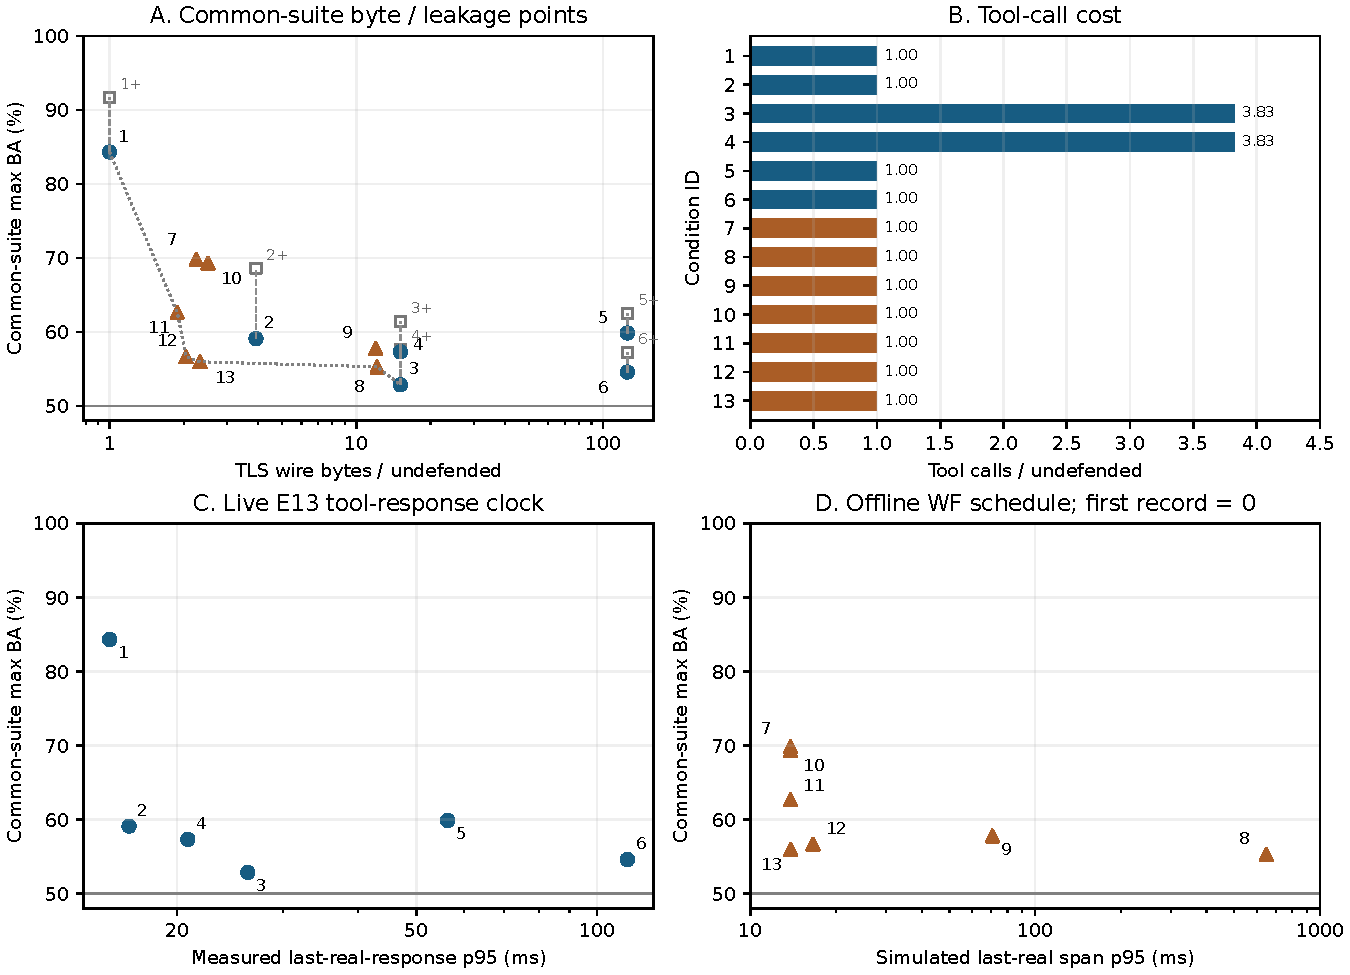
\includegraphics[width=.93\textwidth]{figures/r7-pareto.pdf}
\caption{E14 standard-prompt operating points under the same seven attacks. Labels: 1 undefended, 2 per-call constant, 3 serial shadow, 4 two-in-flight shadow, 5/6 full 2/5\,ms tunnels, 7 record buckets, 8/9 Tamaraw slow/fast, 10 FRONT, 11 WTF-PAD adaptation, 12 random-donor WT, 13 short-calibration FRONT. Gray squares with ``+'' labels in A show larger full-union maxima; dotted nondominance uses only matched colored points and is neither statistically certified nor globally optimal. Circles are measured E13 clocks; triangles are offline transformations. Panels C/D separate time semantics.}
\label{fig:r7-pareto}\end{figure}

Measured delays start at the RPC measurement origin; simulated spans start at the first input record. Zero added delay in FRONT/WTF-PAD's trace transformation does not measure contention on a live link. Actual tool-call ratios remain one for cell-only controls; shadow rows include extra executions. Neither delay panel measures timing-dependent LLM replanning. Thus the byte/BA comparison is shared, while a complete same-scheduler online Pareto comparison remains unperformed.

\subsection{Prospective sample planning}
The planning script varies positive/negative customer counts, assumed BA and attacker dependence using 20,000 binomial trials per setting. It assumes independent customer correctness with equal sensitivity and specificity and a normal 97.5\% upper endpoint, omits the AUROC gate, and is not a power estimate for the observed heterogeneous bootstrap. One attacker also models perfect dependence; seven independent attackers supply a contrasting multiplicity scenario. Under chance-level population BA and three negatives per positive, the searched 80\%-power points are 75 positive customers for one attacker and 150 for seven. Thirty positives is a feasibility floor, not a guaranteed pass. At BA .55, requirements are substantially larger. The planning grid extends the frozen description's 250-customer maximum to 400; this post hoc range extension is recorded in the artifact errata. New independent customer/template sampling must precede a population-level absolute-bound claim.
\begin{table}[ht]\centering\small
\caption{Planning sensitivity: smallest searched positive-cluster count with at least 80\% probability of an upper BA bound below .60. Independent Bernoulli customer correctness and a normal 97.5\% upper endpoint; this omits the AUROC gate and is not the power of the observed heterogeneous bootstrap.}\label{tab:r7-power}
\begin{tabular}{@{}rrrr@{}}\toprule
Negatives per positive & Population BA & Independent attacks & Positive clusters\\\midrule
1 & 0.50 & 1 & 100\\
1 & 0.50 & 7 & 200\\
1 & 0.55 & 1 & 400\\
1 & 0.55 & 7 & $>400$ in grid\\
3 & 0.50 & 1 & 75\\
3 & 0.50 & 7 & 150\\
3 & 0.55 & 1 & 400\\
3 & 0.55 & 7 & $>400$ in grid\\
\bottomrule\end{tabular}\end{table}


The prospective validation file specifies new environment/model versions, precollection customer splits, training-only calibration, the unchanged BA/AUROC gates, live planner utility measurements and blind-human recoding. It is a future protocol, not a completed collection or an external preregistration. Repeated old tasks, a same-provider model extension and AI source review do not satisfy these independent validation requirements.
